\documentclass[aspectratio=169,12pt]{beamer}
\usepackage[utf8]{inputenc}
\usepackage[T1]{fontenc}
\usepackage{amsmath, amssymb}
\usepackage{booktabs}
\usepackage{colortbl}
\usepackage{hyperref}
\usepackage{makecell}
\usepackage{ragged2e}
\usepackage{bytefield}
\usepackage{tikz}
\usetikzlibrary{arrows.meta, positioning, shapes.geometric, calc, tikzmark, shapes.misc, fit, decorations.pathreplacing}
\usepackage[siunitx, RPvoltages]{circuitikz}
\usepackage{tcolorbox}
\usepackage{pgfplots}
\pgfplotsset{compat=1.17}
\usepackage{listings}
\usepackage{xcolor}

\usetheme{Madrid}
\usecolortheme{default}

% Custom colors
\definecolor{mygreen}{RGB}{0,128,0}
\definecolor{myblue}{RGB}{0,0,255}
\definecolor{myred}{RGB}{255,0,0}
\definecolor{techblue}{RGB}{0,56,101}
\definecolor{techgold}{RGB}{177,121,22}
\definecolor{lightgray}{RGB}{240,240,240}

% Code listing style
\lstset{
    basicstyle=\ttfamily\small,
    keywordstyle=\color{blue},
    commentstyle=\color{mygreen},
    stringstyle=\color{myred},
    showstringspaces=false,
    breaklines=true,
    frame=single,
    backgroundcolor=\color{lightgray}
}

\title{Computer Structure}
\subtitle{GPU Architecture and Programming}
\author{Computer Architecture 2360267}
\date{2025, Lecture \#13}

\begin{document}

\frame{\titlepage}

% Table of Contents
\begin{frame}{Outline}
\tableofcontents
\end{frame}

\section{Introduction to GPGPU}

\begin{frame}{What is GPGPU?}
\begin{columns}
\begin{column}{0.6\textwidth}
\textbf{Execute general-purpose compute tasks on GPU}
\begin{itemize}
    \item Massive parallelism
    \item High memory bandwidth
    \item Energy efficiency
    \item Specialized hardware units (e.g., Tensor cores)
\end{itemize}

\vspace{0.3cm}
\textbf{Fits various workloads}
\begin{itemize}
    \item Data-parallel algorithms: linear algebra, FFTs, convolutions
    \item Embarrassingly parallel tasks: Monte Carlo, image/video processing
    \item Batched inference/training in AI/ML pipelines
\end{itemize}
\end{column}

\begin{column}{0.35\textwidth}
\textbf{Mature ecosystem}
\begin{itemize}
    \item APIs: CUDA, OpenCL
    \item Libraries: cuBLAS, cuDNN, Thrust
    \item Frameworks: TensorFlow, PyTorch
\end{itemize}

\vspace{0.3cm}
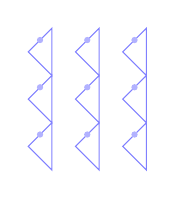
\begin{tikzpicture}[scale=0.4]
\foreach \i in {0,...,2} {
    \foreach \j in {0,...,2} {
        \draw[blue!50] (\i*1.5,\j*1.5) -- ++(0.75,0.75) -- ++(0,-1.5) -- cycle;
        \fill[blue!30] (\i*1.5+0.375,\j*1.5+0.375) circle (0.1);
    }
}
\end{tikzpicture}
\end{column}
\end{columns}
\end{frame}

\begin{frame}{When to Use GPU?}
\begin{columns}
\begin{column}{0.55\textwidth}
\textbf{Arithmetic intensity}
\begin{itemize}
    \item $I = \frac{FLOPs}{bytes\ accessed}$
    \item [bytes accessed] -- usually to slowest memory only
    \item \textbf{$I \gtrsim 5$--10 FLOP/byte}

    $\rightarrow$ Almost certainly \textbf{compute-bound} on modern GPUs (e.g. H100)
    \item Also known as ``Operational Intensity''
\end{itemize}
\end{column}

\begin{column}{0.4\textwidth}
\textbf{Sometimes can benefit even with low AI:}
\begin{itemize}
    \item \textbf{Massive parallelism} hides latency
    \item \textbf{High-throughput HBM}
    \item \textbf{Overlap} of compute \& memory
\end{itemize}
\end{column}
\end{columns}
\end{frame}

\begin{frame}{Roofline Model}
\begin{columns}
\begin{column}{0.5\textwidth}
\small
\textbf{Visual model for estimating performance}
\begin{itemize}
    \item Targets multi-core, many-core, accelerator architectures
    \item Highlights hardware limits and guides optimization priorities
\end{itemize}

\textbf{Combines:}
\begin{itemize}
    \item Maximum performance ($\pi$)
    \item Arithmetic intensity (I)
    \item Memory bandwidth ($\beta$)
\end{itemize}

\textbf{Assesses performance quality}

\vspace{0.2cm}
$P = \min\left\{\pi, \beta \cdot I\right\}$
\end{column}

\begin{column}{0.45\textwidth}
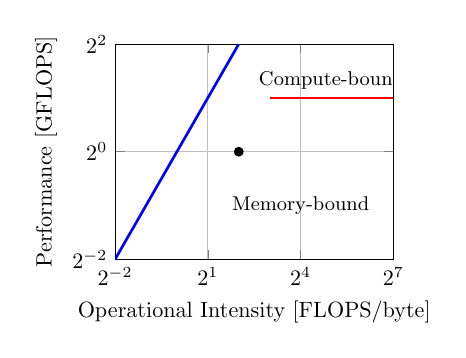
\begin{tikzpicture}[scale=0.8]
    \begin{axis}[
        xlabel={Operational Intensity [FLOPS/byte]},
        ylabel={Performance [GFLOPS]},
        xmode=log,
        ymode=log,
        log basis x={2},
        log basis y={2},
        xmin=0.25, xmax=128,
        ymin=0.25, ymax=4,
        grid=major,
        width=6cm,
        height=5cm,
        legend pos=south east
    ]
    % Memory bandwidth bound line
    \addplot[blue, very thick, domain=0.25:8] {x};
    % Compute bound horizontal line
    \addplot[red, very thick, domain=8:128] {2};
    % Example point
    \addplot[mark=*, mark size=2pt] coordinates {(4,1)};
    \node at (axis cs:16,0.5) {\small Memory-bound};
    \node at (axis cs:32,2.5) {\small Compute-bound};
    \end{axis}
\end{tikzpicture}
\end{column}
\end{columns}
\end{frame}

\section{GPU Architecture}

\begin{frame}{NVIDIA H100 Architecture (Hopper)}
\begin{center}
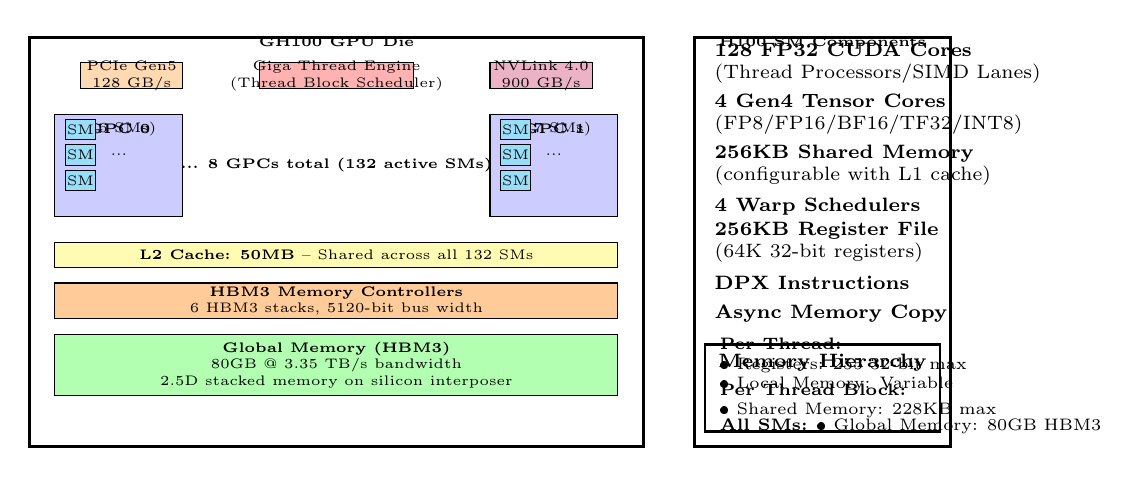
\begin{tikzpicture}[scale=0.65, every node/.style={font=\tiny}]
% Main die outline
\draw[very thick] (0,0) rectangle (12,8);
\node[anchor=north] at (6,8.2) {\textbf{GH100 GPU Die}};

% Top controllers
\draw[fill=orange!30] (1,7) rectangle (3,7.5);
\node[align=center] at (2,7.25) {PCIe Gen5\\128 GB/s};

\draw[fill=red!30] (4.5,7) rectangle (7.5,7.5);
\node[align=center] at (6,7.25) {Giga Thread Engine\\(Thread Block Scheduler)};

\draw[fill=purple!30] (9,7) rectangle (11,7.5);
\node[align=center] at (10,7.25) {NVLink 4.0\\900 GB/s};

% GPCs - left side
\draw[fill=blue!20] (0.5,4.5) rectangle (3,6.5);
\node[anchor=north] at (1.75,6.5) {\textbf{GPC 0}};
\node at (1.75,6.2) {(16 SMs)};
\foreach \i in {1,...,3} {
    \draw[fill=cyan!40] (0.7,4.5+\i*0.5) rectangle (1.3,4.9+\i*0.5);
    \node[font=\fontsize{5}{6}\selectfont] at (1,4.7+\i*0.5) {SM};
}
\node at (1.75,5.7) {...};

% GPCs - right side
\draw[fill=blue!20] (9,4.5) rectangle (11.5,6.5);
\node[anchor=north] at (10.25,6.5) {\textbf{GPC 1}};
\node at (10.25,6.2) {(17 SMs)};
\foreach \i in {1,...,3} {
    \draw[fill=cyan!40] (9.2,4.5+\i*0.5) rectangle (9.8,4.9+\i*0.5);
    \node[font=\fontsize{5}{6}\selectfont] at (9.5,4.7+\i*0.5) {SM};
}
\node at (10.25,5.7) {...};

\node at (6,5.5) {\textbf{... 8 GPCs total (132 active SMs)}};

% L2 Cache
\draw[fill=yellow!30] (0.5,3.5) rectangle (11.5,4);
\node at (6,3.75) {\textbf{L2 Cache: 50MB} -- Shared across all 132 SMs};

% Memory controllers
\draw[fill=orange!40] (0.5,2.5) rectangle (11.5,3.2);
\node[align=center] at (6,2.85) {\textbf{HBM3 Memory Controllers}\\6 HBM3 stacks, 5120-bit bus width};

% Global memory
\draw[fill=green!30] (0.5,1) rectangle (11.5,2.2);
\node[align=center] at (6,1.6) {\textbf{Global Memory (HBM3)}\\80GB @ 3.35 TB/s bandwidth\\2.5D stacked memory on silicon interposer};

% SM Components box (right side)
\draw[very thick] (13,0) rectangle (18,8);
\node[anchor=north] at (15.5,8.2) {\textbf{H100 SM Components}};

\node[anchor=west, align=left, font=\fontsize{7}{8}\selectfont] at (13.2,7.5) {
\textbf{128 FP32 CUDA Cores}\\
(Thread Processors/SIMD Lanes)
};

\node[anchor=west, align=left, font=\fontsize{7}{8}\selectfont] at (13.2,6.5) {
\textbf{4 Gen4 Tensor Cores}\\
(FP8/FP16/BF16/TF32/INT8)
};

\node[anchor=west, align=left, font=\fontsize{7}{8}\selectfont] at (13.2,5.5) {
\textbf{256KB Shared Memory}\\
(configurable with L1 cache)
};

\node[anchor=west, align=left, font=\fontsize{7}{8}\selectfont] at (13.2,4.7) {
\textbf{4 Warp Schedulers}
};

\node[anchor=west, align=left, font=\fontsize{7}{8}\selectfont] at (13.2,4) {
\textbf{256KB Register File}\\
(64K 32-bit registers)
};

\node[anchor=west, align=left, font=\fontsize{7}{8}\selectfont] at (13.2,3.2) {
\textbf{DPX Instructions}
};

\node[anchor=west, align=left, font=\fontsize{7}{8}\selectfont] at (13.2,2.6) {
\textbf{Async Memory Copy}
};

% Memory hierarchy box
\draw[thick] (13.2,0.3) rectangle (17.8,2);
\node[anchor=north, font=\fontsize{7}{8}\selectfont] at (15.5,2) {\textbf{Memory Hierarchy}};
\node[anchor=west, align=left, font=\fontsize{6}{7}\selectfont] at (13.3,1.6) {
\textbf{Per Thread:}\\
• Registers: 255 32-bit max\\
• Local Memory: Variable
};
\node[anchor=west, align=left, font=\fontsize{6}{7}\selectfont] at (13.3,0.9) {
\textbf{Per Thread Block:}\\
• Shared Memory: 228KB max
};
\node[anchor=west, align=left, font=\fontsize{6}{7}\selectfont] at (13.3,0.4) {
\textbf{All SMs:} • Global Memory: 80GB HBM3
};

\end{tikzpicture}
\end{center}
\end{frame}

\begin{frame}{Graphics Processing Cluster (GPC)}
\textbf{GPC - Graphics Processing Cluster}
\begin{itemize}
    \item Several \textbf{SMs} (Streaming Multiprocessors), each running warps of threads
    \item Texture units, raster engines, and L2 cache interfaces
    \item Not exposed to software
\end{itemize}

\vspace{0.5cm}
\textbf{Memory-access patterns that cross GPC boundaries} (e.g. very large shared-memory tiling) may see slightly different latency/GPU-internal routing
\end{frame}

\begin{frame}{CUDA Compilation Flow}
\begin{columns}
\begin{column}{0.55\textwidth}
\begin{itemize}
    \item Code is compiled into \textbf{PTX code} (intermediate representation)
    \item Then optimized to the specific GPU
    \begin{itemize}
        \item Offline (specific GPU given)
        \item JIT
    \end{itemize}
    \item PTX resembles GPU instruction set but not identical
    \begin{itemize}
        \item GPU peculiarities hidden
    \end{itemize}
    \item Use (PTX) intrinsics for performance
\end{itemize}
\end{column}

\begin{column}{0.4\textwidth}
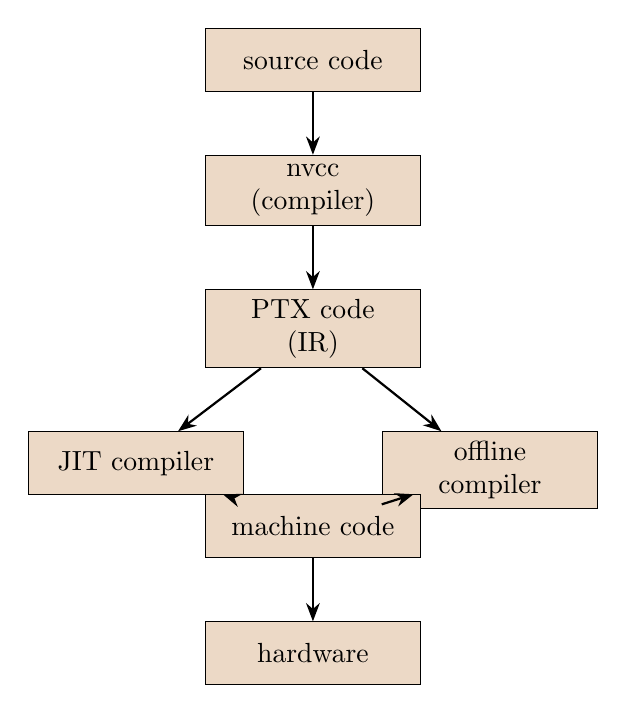
\begin{tikzpicture}[
    node distance=0.8cm,
    box/.style={rectangle, draw, fill=brown!30, text width=2.5cm, align=center, minimum height=0.8cm},
    arrow/.style={->, >=Stealth, thick}
]
\node[box] (source) {source code};
\node[box, below=of source] (nvcc) {nvcc\\(compiler)};
\node[box, below=of nvcc] (ptx) {PTX code\\(IR)};
\node[box, below left=0.8cm and -0.5cm of ptx] (jit) {JIT compiler};
\node[box, below right=0.8cm and -0.5cm of ptx] (offline) {offline\\compiler};
\node[box, below=1.6cm of ptx] (machine) {machine code};
\node[box, below=of machine] (hardware) {hardware};

\draw[arrow] (source) -- (nvcc);
\draw[arrow] (nvcc) -- (ptx);
\draw[arrow] (ptx) -- (jit);
\draw[arrow] (ptx) -- (offline);
\draw[arrow] (jit) -- (machine);
\draw[arrow] (offline) -- (machine);
\draw[arrow] (machine) -- (hardware);
\end{tikzpicture}
\end{column}
\end{columns}
\end{frame}

\section{Compute}

\begin{frame}{GPU Scheduler}
\begin{columns}
\begin{column}{0.48\textwidth}
\textbf{Grid \& Block Dispatch}
\begin{itemize}
    \item Kernel $\rightarrow$ grid of blocks (array of vectorizable loops)
    \item SMs pull blocks when resources (registers/shared mem) free
\end{itemize}

\textbf{Warp Scheduling Inside SMs}
\begin{itemize}
    \item Threads grouped into 32-thread warps
    \item Warp scheduler issues ready warps round-robin (probably) to hide stalls
\end{itemize}

\textbf{Occupancy Impact:}
\begin{itemize}
    \item Occupancy = active warps / max warps per SM
\end{itemize}
\end{column}

\begin{column}{0.48\textwidth}
\textbf{Latency Hiding}
\begin{itemize}
    \item High block occupancy $\Rightarrow$ many warps queued
    \item When one warp stalls (e.g. memory), another executes
\end{itemize}

\textbf{Resource Constraints}
\begin{itemize}
    \item Block-level: limited by per-SM registers \& shared memory
    \item Warp-level: limited by per-thread registers (max 255) and active warps
\end{itemize}

\textbf{Tune for Balance}
\begin{itemize}
    \item Choose block size to maximize occupancy
    \item Limit registers/thread to feed warp scheduler without causing spills
\end{itemize}
\end{column}
\end{columns}
\end{frame}

\begin{frame}[fragile]{SM Architecture \& Warp Scheduling}
\begin{center}
\scalebox{0.7}{
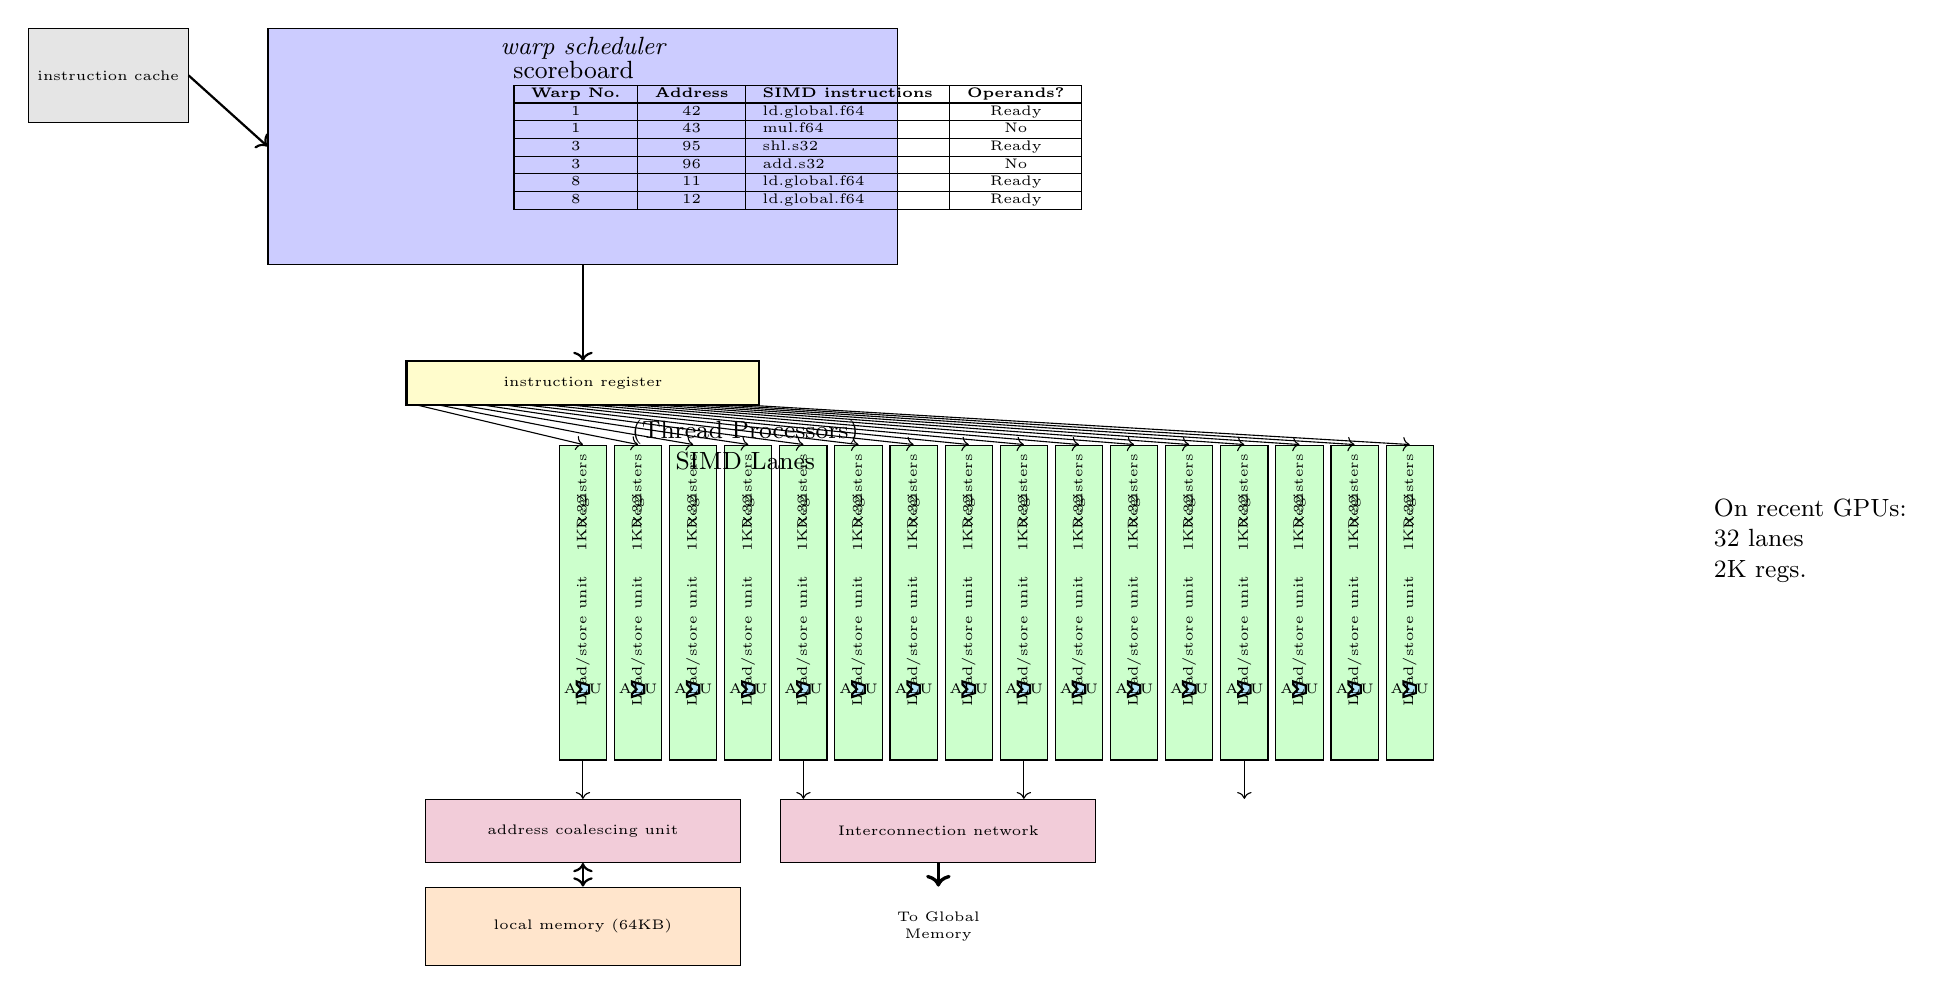
\begin{tikzpicture}[
    every node/.style={font=\tiny},
    box/.style={draw, fill=#1, minimum height=1cm},
    box/.default=gray!20
]

% Instruction cache
\node[box, minimum width=2cm, minimum height=1.2cm] (icache) at (0,0) {instruction cache};

% Warp scheduler box
\node[box=blue!20, minimum width=8cm, minimum height=3cm, anchor=north west]
    (scheduler) at ([xshift=1cm]icache.north east) {};
\node[anchor=north, font=\small\itshape] at (scheduler.north) {warp scheduler};

% Scoreboard label
\node[anchor=north west, font=\small] at ([xshift=3cm, yshift=-0.3cm]scheduler.north west) {scoreboard};

% Scoreboard table in minipage
\node[anchor=north west, yshift=-0.6cm] at ([xshift=3cm]scheduler.north west) {
\begin{minipage}{6cm}
\tiny
\begin{tabular}{|c|c|l|c|}
\hline
\textbf{Warp No.} & \textbf{Address} & \textbf{SIMD instructions} & \textbf{Operands?} \\
\hline
1 & 42 & ld.global.f64 & Ready \\
\hline
1 & 43 & mul.f64 & No \\
\hline
3 & 95 & shl.s32 & Ready \\
\hline
3 & 96 & add.s32 & No \\
\hline
8 & 11 & ld.global.f64 & Ready \\
\hline
8 & 12 & ld.global.f64 & Ready \\
\hline
\end{tabular}
\end{minipage}
};

% Arrow from instruction cache to scheduler
\draw[->, thick] (icache.east) -- (scheduler.west);

% Instruction register (muxdemux)
\node[muxdemux, muxdemux def={Rh=1, Lh=1, w=8, NT=1, NB=16, square pins=1},
      external pins width=0, fill=yellow!20, font=\tiny]
    (ireg) at ([yshift=-1.5cm]scheduler.south) {instruction register};

% Arrow from scheduler to instruction register
\draw[->, thick] (scheduler.south) -- (ireg.tpin 1);

% SIMD lanes container
\coordinate (lanes-start) at ([yshift=-0.5cm]ireg.south);

% SIMD lanes using foreach
\foreach \i in {0,...,15} {
    \coordinate (lane\i) at ([xshift=\i*0.7cm]lanes-start);

    % Lane container as node
    \node[box=green!20, minimum width=0.6cm, minimum height=4cm, anchor=north, inner sep=0]
        (lane\i-box) at (lane\i) {};

    % Registers section
    \node[rotate=90, font=\fontsize{5}{6}\selectfont] at ([yshift=-0.6cm]lane\i-box.north) {Registers};
    \node[rotate=90, font=\fontsize{5}{6}\selectfont] at ([yshift=-1cm]lane\i-box.north) {1K×32};

    % Load/store unit
    \node[rotate=90, font=\fontsize{5}{6}\selectfont] at ([yshift=-2.5cm]lane\i-box.north) {Load/store unit};

    % ALU (muxdemux with inset for trapezoid shape)
    \node[muxdemux, muxdemux def={Lh=1, Rh=0.5, w=0.8, inset w=0.3, inset Lh=0.6, inset Rh=0, square pins=1},
          external pins width=0, fill=cyan!30, scale=0.35]
        (lane\i-alu) at ([yshift=-1.1cm]lane\i-box.center) {};
    \node[font=\fontsize{4}{5}\selectfont] at (lane\i-alu.center) {ALU};

    % Arrow from instruction register bottom pin to lane
    \pgfmathtruncatemacro{\pinnum}{\i+1}
    \draw[->, thin] (ireg.bpin \pinnum) -- (lane\i-box.north);
}

% Label for lanes
\node[anchor=west, font=\small, align=center] at ([xshift=0.5cm]lanes-start)
    {(Thread Processors)\\SIMD Lanes};

% Address coalescing unit
\node[box=purple!20, minimum width=4cm, minimum height=0.8cm, anchor=north]
    (coalesce) at ([yshift=-4.5cm]lanes-start) {address coalescing unit};

% Interconnection network
\node[box=purple!20, minimum width=4cm, minimum height=0.8cm, anchor=north west]
    (interconnect) at ([xshift=0.5cm]coalesce.north east) {Interconnection network};

% Arrows from some lanes to coalescing unit
\foreach \i in {0,4,8,12} {
    \draw[->, thin] (lane\i-box.south) -- (lane\i-box.south |- coalesce.north);
}

% Local memory
\node[box=orange!20, minimum width=4cm, minimum height=1cm, anchor=north]
    (localmem) at ([yshift=-0.3cm]coalesce.south) {local memory (64KB)};

% Arrow between coalescing and local memory
\draw[<->, thick] (coalesce.south) -- (localmem.north);

% To global memory label
\node[anchor=north, align=center] at ([yshift=-0.5cm]interconnect.south)
    {To Global\\Memory};
\draw[->, very thick] (interconnect.south) -- ([yshift=-0.3cm]interconnect.south);

% Note about recent GPUs
\node[anchor=west, font=\small, align=left] at ([xshift=12cm, yshift=-2cm]ireg.east)
    {On recent GPUs:\\32 lanes\\2K regs.};

\end{tikzpicture}
}
\end{center}
\end{frame}

\begin{frame}{Registers}
\begin{columns}
\begin{column}{0.48\textwidth}
\textbf{Limited On-Chip Resource:} Each SM has a fixed register file (e.g., 64K registers on many NVIDIA GPUs)
\begin{itemize}
    \item Each thread can use at most 255 registers
\end{itemize}

\textbf{Latency Hiding vs. Resource Use:}
\begin{itemize}
    \item Registers per thread directly cap the number of resident warps
    \item High occupancy helps hide memory latency
    \item Excessive register use improves ILP
    \item ... but may starve the SM of parallel work
\end{itemize}
\end{column}

\begin{column}{0.48\textwidth}
\textbf{Tuning Registers:}
\begin{itemize}
    \item Use \texttt{-maxrregcount} or \texttt{\_\_launch\_bounds\_\_()} to limit registers/thread
    \item Balance between enough registers for compute
    \item ... and enough threads for latency hiding
\end{itemize}

\textbf{Register spilling}
\begin{itemize}
    \item Spilling when a kernel's register demand exceeds either the hardware limit (255/thread) or the compiler-set limit
    \item 100s of cycles penalty
    \item Refactor code to reuse variables and reduce live ranges
    \item ... or lower occupancy
\end{itemize}
\end{column}
\end{columns}
\end{frame}

\begin{frame}{GPU Warp Divergence}
\begin{columns}
\begin{column}{0.45\textwidth}
\textbf{Conditional Branch:} An if-statement can cause threads to diverge
\begin{itemize}
    \item Some threads take ``true'' path
    \item Others take the ``false'' path
    \item PC and active mask are pushed into a stack
    \item Code execution is \textbf{serialized}
\end{itemize}

\vspace{0.3cm}
\textbf{Convergence:} Both paths merge back together, and all threads become active again
\end{column}

\begin{column}{0.5\textwidth}
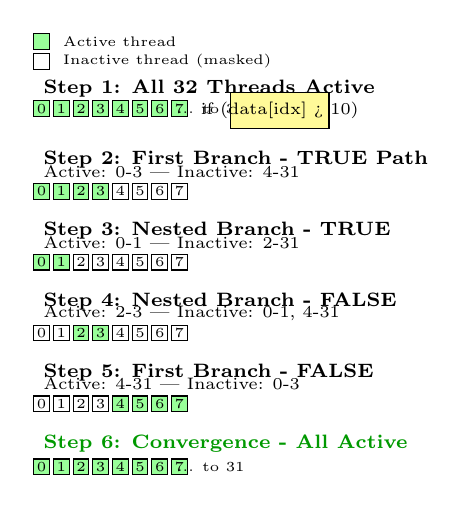
\begin{tikzpicture}[scale=0.5, every node/.style={font=\tiny}]
% Legend
\draw[fill=green!40] (0,9) rectangle (0.4,9.4);
\node[anchor=west] at (0.5,9.2) {Active thread};
\draw[fill=white] (0,8.5) rectangle (0.4,8.9);
\node[anchor=west] at (0.5,8.7) {Inactive thread (masked)};

% Step 1
\node[anchor=west, font=\fontsize{7}{8}\selectfont] at (0,8) {\textbf{Step 1: All 32 Threads Active}};
\foreach \i in {0,...,7} {
    \draw[fill=green!40] (\i*0.5,7.3) rectangle (\i*0.5+0.4,7.7);
    \node at (\i*0.5+0.2,7.5) {\i};
}
\node at (4.5,7.5) {... to 31};
\draw[fill=yellow!40] (5,7) rectangle (7.5,7.9);
\node[align=center, font=\fontsize{6}{7}\selectfont] at (6.25,7.45) {if (data[idx] > 10)};

% Step 2
\node[anchor=west, font=\fontsize{7}{8}\selectfont] at (0,6.2) {\textbf{Step 2: First Branch - TRUE Path}};
\node[anchor=west, font=\fontsize{6}{7}\selectfont] at (0,5.9) {Active: 0-3 | Inactive: 4-31};
\foreach \i in {0,...,3} {
    \draw[fill=green!40] (\i*0.5,5.2) rectangle (\i*0.5+0.4,5.6);
    \node at (\i*0.5+0.2,5.4) {\i};
}
\foreach \i in {4,...,7} {
    \draw[fill=white] (\i*0.5,5.2) rectangle (\i*0.5+0.4,5.6);
    \node at (\i*0.5+0.2,5.4) {\i};
}

% Step 3
\node[anchor=west, font=\fontsize{7}{8}\selectfont] at (0,4.4) {\textbf{Step 3: Nested Branch - TRUE}};
\node[anchor=west, font=\fontsize{6}{7}\selectfont] at (0,4.1) {Active: 0-1 | Inactive: 2-31};
\foreach \i in {0,...,1} {
    \draw[fill=green!40] (\i*0.5,3.4) rectangle (\i*0.5+0.4,3.8);
    \node at (\i*0.5+0.2,3.6) {\i};
}
\foreach \i in {2,...,7} {
    \draw[fill=white] (\i*0.5,3.4) rectangle (\i*0.5+0.4,3.8);
    \node at (\i*0.5+0.2,3.6) {\i};
}

% Step 4
\node[anchor=west, font=\fontsize{7}{8}\selectfont] at (0,2.6) {\textbf{Step 4: Nested Branch - FALSE}};
\node[anchor=west, font=\fontsize{6}{7}\selectfont] at (0,2.3) {Active: 2-3 | Inactive: 0-1, 4-31};
\foreach \i in {0,...,1} {
    \draw[fill=white] (\i*0.5,1.6) rectangle (\i*0.5+0.4,2.0);
    \node at (\i*0.5+0.2,1.8) {\i};
}
\foreach \i in {2,...,3} {
    \draw[fill=green!40] (\i*0.5,1.6) rectangle (\i*0.5+0.4,2.0);
    \node at (\i*0.5+0.2,1.8) {\i};
}
\foreach \i in {4,...,7} {
    \draw[fill=white] (\i*0.5,1.6) rectangle (\i*0.5+0.4,2.0);
    \node at (\i*0.5+0.2,1.8) {\i};
}

% Step 5
\node[anchor=west, font=\fontsize{7}{8}\selectfont] at (0,0.8) {\textbf{Step 5: First Branch - FALSE}};
\node[anchor=west, font=\fontsize{6}{7}\selectfont] at (0,0.5) {Active: 4-31 | Inactive: 0-3};
\foreach \i in {0,...,3} {
    \draw[fill=white] (\i*0.5,-0.2) rectangle (\i*0.5+0.4,0.2);
    \node at (\i*0.5+0.2,0) {\i};
}
\foreach \i in {4,...,7} {
    \draw[fill=green!40] (\i*0.5,-0.2) rectangle (\i*0.5+0.4,0.2);
    \node at (\i*0.5+0.2,0) {\i};
}

% Step 6
\node[anchor=west, font=\fontsize{7}{8}\selectfont, color=green!60!black] at (0,-1) {\textbf{Step 6: Convergence - All Active}};
\foreach \i in {0,...,7} {
    \draw[fill=green!40] (\i*0.5,-1.8) rectangle (\i*0.5+0.4,-1.4);
    \node at (\i*0.5+0.2,-1.6) {\i};
}
\node at (4.5,-1.6) {... to 31};
\end{tikzpicture}
\end{column}
\end{columns}
\end{frame}

\begin{frame}{GPU Warp Divergence: Solutions}
\begin{columns}
\begin{column}{0.6\textwidth}
\textbf{Data reorganization}
\begin{itemize}
    \item Sort/group data so threads in a warp take the same branch
\end{itemize}

\textbf{Predicated instructions}
\begin{itemize}
    \item Instead of short branches (< 7 instructions)
    \item Can waste cycles if used unnecessarily
    \item Compiler will usually do that
\end{itemize}

\textbf{Separate kernels}
\begin{itemize}
    \item Extreme cases
\end{itemize}

\textbf{Algorithmic restructuring}
\begin{itemize}
    \item Replace branches with arithmetic
\end{itemize}

\textbf{Warp-level primitives}
\begin{itemize}
    \item E.g., reduction using \texttt{\_\_shfl\_down\_sync}
\end{itemize}
\end{column}

\begin{column}{0.35\textwidth}
\begin{tcolorbox}[colback=lightgray, colframe=black, title=Arithmetic replacement]
\texttt{\small
result = condition * trueValue + (!condition) * falseValue;
}
\end{tcolorbox}

\vspace{0.3cm}
\begin{tcolorbox}[colback=lightgray, colframe=black, title=Warp reduction]
\texttt{\tiny
\#define FULL\_MASK 0xffffffff\\
for (int offset = 16; offset > 0; offset /= 2)\\
\ \ val += \_\_shfl\_down\_sync(FULL\_MASK, val, offset);
}
\end{tcolorbox}
\end{column}
\end{columns}
\end{frame}

\begin{frame}{Kernel Fusion and Fission}
\begin{columns}
\begin{column}{0.48\textwidth}
\textbf{Kernel Fusion} combines multiple sequential kernels into a single launch
\begin{itemize}
    \item Reduces \textbf{kernel launch overhead}
    \item Reduces global memory traffic by \textbf{reusing data} in registers/shared memory
    \item May \textcolor{red}{increase register pressure} and code complexity, potentially limiting occupancy
\end{itemize}
\end{column}

\begin{column}{0.48\textwidth}
\textbf{Kernel Fission} splits a large kernel into smaller, more focused kernels
\begin{itemize}
    \item Lowers register and shared-memory usage per kernel, \textbf{improving occupancy} and load balancing
    \item Exposes \textbf{finer-grained parallelism} and simplifies optimization of individual stages
    \item Incurs \textcolor{red}{extra launches} and memory transfers, which can offset fission benefits if over-applied
\end{itemize}
\end{column}
\end{columns}

\vspace{0.3cm}
\textbf{Usually done manually}
\begin{itemize}
    \item Some automation by libraries/frameworks
\end{itemize}
\end{frame}

\begin{frame}{DPX (Dynamic Programming eXtensions)}
\textbf{DPX is a set of specialized fused-compute instructions}
\begin{itemize}
    \item Enable finding min and max values
    \item \& fused addition and min/max
    \item Up to three 16 and 32-bit signed or unsigned integer parameters
    \item Optional ReLU (clamping to zero)
\end{itemize}

\vspace{0.3cm}
\textbf{Can be used by compiler / intrinsic}

\vspace{0.5cm}
\textbf{Example: Floyd--Warshall Algorithm}
\begin{itemize}
    \item Find the lengths (summed weights) of shortest paths between all pairs of vertices
    \item Useful in robotics
    \item \texttt{dist[i][j] = min(dist[i][j], dist[i][k] + dist[k][j])}
    \item Can use DPX instruction for fused min+add
\end{itemize}
\end{frame}

\begin{frame}{Tensor Cores}
\textbf{Tensors:} multi-dimensional arrays

\textbf{Warp Matrix Multiply Accumulate (WMMA)}

\textbf{Frameworks} like \textbf{cuBLAS, cuDNN, PyTorch}, and \textbf{TensorFlow} internally use WMMA to speed up operations like matmul, conv2d, and transformer attention blocks.

\vspace{0.3cm}
\textbf{Tensor Cores:} Specialized for matrix multiply-accumulate (MMA) operations
\begin{itemize}
    \item Operates on small fixed-size matrices (e.g., 16×16×16)
    \item Performs $D = A \times B + C$ at hardware speed
\end{itemize}

\vspace{0.3cm}
\textbf{Supported precisions:}
\begin{itemize}
    \item FP16 (IEEE half-precision): 1 sign, 5 exponent, 10 mantissa
    \item BF16 (Brain Float): 1 sign, 8 exponent, 7 mantissa -- same range as FP32
    \item TF32 (Tensor Float): uses FP32 inputs but internally truncates to 10-bit mantissa
    \item INT8/INT4 for quantized inference
    \item Accumulator precision is almost always \textbf{FP32}
\end{itemize}
\end{frame}

\begin{frame}{WMMA: Row-major vs. Column-major}
\begin{columns}
\begin{column}{0.55\textwidth}
\textbf{Row-major vs. column-major}

CUDA C/C++ default is \textbf{row-major}: elements A[i][j] are laid out so that A[i][j] and A[i][j+1] are contiguous in memory.

\vspace{0.3cm}
WMMA fragments can be declared for either layout (\texttt{row\_major} or \texttt{col\_major}), but you must match your data's layout.
\end{column}

\begin{column}{0.4\textwidth}
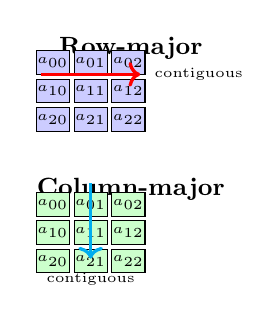
\begin{tikzpicture}[scale=0.6]
% Row-major
\node[anchor=north] at (2,3.5) {\small\textbf{Row-major}};
\foreach \i in {0,1,2} {
    \foreach \j in {0,1,2} {
        \draw[fill=blue!20] (\j*0.8,3-\i*0.6) rectangle (\j*0.8+0.7,3-\i*0.6-0.5);
        \node[font=\tiny] at (\j*0.8+0.35,3-\i*0.6-0.25) {$a_{\i\j}$};
    }
}
\draw[->, red, very thick] (0.1,2.5) -- (2.2,2.5);
\node[right, font=\tiny] at (2.3,2.5) {contiguous};

% Column-major
\node[anchor=north] at (2,0.5) {\small\textbf{Column-major}};
\foreach \i in {0,1,2} {
    \foreach \j in {0,1,2} {
        \draw[fill=green!20] (\j*0.8,0-\i*0.6) rectangle (\j*0.8+0.7,0-\i*0.6-0.5);
        \node[font=\tiny] at (\j*0.8+0.35,0-\i*0.6-0.25) {$a_{\i\j}$};
    }
}
\draw[->, cyan, very thick] (1.15,0.2) -- (1.15,-1.4);
\node[below, font=\tiny] at (1.15,-1.5) {contiguous};
\end{tikzpicture}
\end{column}
\end{columns}
\end{frame}

\begin{frame}{Quantization}
\begin{columns}
\begin{column}{0.55\textwidth}
\textbf{Converting high-precision model parameters} (e.g., 32-bit floats) into lower-precision formats (e.g., 8-bit integers) to reduce compute and memory requirements.

\vspace{0.3cm}
\textbf{Benefits:}
\begin{itemize}
    \item Lowers memory footprint
    \item Speeds up inference
    \item Enables deployment on resource-constrained hardware
\end{itemize}

\textbf{Potential accuracy loss}
\end{column}

\begin{column}{0.4\textwidth}
\textbf{Common Quantization Schemes}
\begin{itemize}
    \item \textbf{Post-Training Quantization (PTQ):} Quantize a fully trained model without retraining
    \item \textbf{Quantization-Aware Training (QAT):} Simulate quantization effects during training to preserve accuracy
\end{itemize}
\end{column}
\end{columns}
\end{frame}

\section{GPU and Memory}

\begin{frame}{HBM (High Bandwidth Memory)}
\begin{columns}
\begin{column}{0.5\textwidth}
\textbf{3D-stacked DRAM architecture}
\begin{itemize}
    \item Places memory dies vertically atop a base logic die
    \item Interconnected via through-silicon vias (TSVs)
\end{itemize}

\vspace{0.3cm}
\textbf{Benefits:}
\begin{itemize}
    \item Massive bandwidth, low latency
    \item Wide interface (1024+ bits)
    \item Low power per bit
\end{itemize}
\end{column}

\begin{column}{0.45\textwidth}
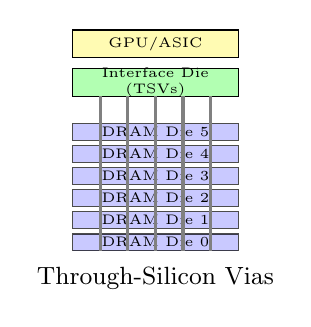
\begin{tikzpicture}[scale=0.7]
% HBM stack illustration
\foreach \i in {0,...,5} {
    \draw[fill=blue!30, opacity=0.7] (0,\i*0.4) rectangle (3,\i*0.4+0.3);
    \node[font=\tiny] at (1.5,\i*0.4+0.15) {DRAM Die \i};
}
\draw[fill=green!30] (0,2.8) rectangle (3,3.3);
\node[font=\tiny, align=center] at (1.5,3.05) {Interface Die\\(TSVs)};

\draw[fill=yellow!30] (0,3.5) rectangle (3,4);
\node[font=\tiny] at (1.5,3.75) {GPU/ASIC};

% TSV illustration
\foreach \i in {0.5,1,1.5,2,2.5} {
    \draw[very thick, gray] (\i,0) -- (\i,2.8);
}

\node[font=\small] at (1.5,-0.5) {Through-Silicon Vias};
\end{tikzpicture}
\end{column}
\end{columns}
\end{frame}

\begin{frame}{Different Memory Types}
\tiny
\begin{tabular}{|l|c|c|c|c|c|}
\hline
\textbf{Parameter} & \textbf{LPDDR4x} & \textbf{LPDDR5} & \textbf{DDR4} & \textbf{GDDR6} & \textbf{HBM2E} \\
\hline
Bandwidth (Gbps) & Low-Med (136) & Med (204) & Med (200) & High (512) & \textbf{Highest (3686)} \\
\hline
Data Rate (Gbps) & 4.266 & 6.4 & 3.2 & 16 & 3.6 \\
\hline
Interface Width (bits) & 32 & 32 & 64 & 32 & \textbf{1024} \\
\hline
Board Area / Design & Large/Med & Med/Med & Large/Easy & Med/Med & Small/Complex \\
\hline
Efficiency (mW/Gbps) & High (3) & High (3) & Mod (10) & Mod (10) & \textbf{Highest (2)} \\
\hline
Cost & Medium & Medium & \textbf{Low} & Medium & High \\
\hline
Reliability/Yield & Good & Good & Good & Good & Moderate \\
\hline
Applications & Mobile, AI & Mobile, AI & Compute & AI, Graphics & AI, HPC \\
\hline
\end{tabular}

\vspace{0.3cm}
\normalsize
Key insight: HBM achieves highest bandwidth through \textbf{wide interface} (1024 bits) × moderate data rate (3.6 Gbps) = 3686 Gbps total
\end{frame}

\begin{frame}{Asynchronous Memory Copying}
\small
\textbf{Host $\rightarrow$ Device DMA}
\begin{itemize}
    \item GPU DMA engines can transfer data over PCIe/NVLink without CPU intervention
    \item \texttt{cudaMemcpyAsync()} issues non-blocking transfers on a copy engine, overlapping PCIe/NVLink traffic with compute on separate streams
\end{itemize}

\textbf{Device-Side Global $\rightarrow$ Shared}
\begin{itemize}
    \item \texttt{cp.async} (or \texttt{cuda::memcpy\_async}) enqueues transfers into a hardware FIFO
    \item Data movement is decoupled from warp execution
\end{itemize}

\textbf{Pipelining \& Overlap}
\begin{itemize}
    \item Use multi-stage pipelines (double-buffering) or the CUDA C++ \texttt{cuda::pipeline} API
    \item Issue next-tile copies before consuming current data
    \item Hides hundreds of cycles of global-memory latency behind active computation
\end{itemize}

\textbf{Best Practices}
\begin{itemize}
    \item Allocate host buffers with \texttt{cudaHostAlloc} for true async host-to-device DMA
    \item Align and tile data to cache-line boundaries for maximal throughput
    \item Balance pipeline depth (stages) with shared-memory footprint and occupancy
\end{itemize}
\end{frame}

\begin{frame}[fragile]{Pipelining Example: Single Stage}
\begin{lstlisting}[language=C++, basicstyle=\ttfamily\fontsize{5}{6}\selectfont]
__global__ void with_single_stage(int* global_out, int const* global_in,
                                   size_t size, size_t batch_sz) {
  auto block = cooperative_groups::this_thread_block();
  constexpr size_t stages_count = 1;
  extern __shared__ int shared[];

  __shared__ cuda::pipeline_shared_state<
    cuda::thread_scope::thread_scope_block, stages_count> shared_state;
  auto pipeline = cuda::make_pipeline(block, &shared_state);

  for (size_t batch = 0; batch < batch_sz; ++batch) {
    // Acquire pipeline stage
    pipeline.producer_acquire();

    // Submit async copy to pipeline's head stage
    cuda::memcpy_async(block, shared, global_in + block_batch(batch),
                       sizeof(int) * block.size(), pipeline);

    // Commit (advance) the pipeline's head stage
    pipeline.producer_commit();

    // Wait for operations to complete
    pipeline.consumer_wait();

    // Computation overlapped with memcpy_async
    compute(global_out + block_batch(batch), shared);

    // Release stage resources
    pipeline.consumer_release();
  }
}
\end{lstlisting}
\end{frame}

\begin{frame}[fragile]{Pipelining Example: Multi-Stage}
\begin{lstlisting}[language=C++, basicstyle=\ttfamily\fontsize{5}{6}\selectfont]
template <size_t stages_count = 2>
__global__ void with_staging(int* global_out, int const* global_in,
                              size_t size, size_t batch_sz) {
  extern __shared__ int shared[]; // stages_count * block.size() elements

  for (size_t compute_batch = 0, fetch_batch = 0;
       compute_batch < batch_sz; ++compute_batch) {
    // Inner loop: fill pipeline with multiple stages
    for (; fetch_batch < batch_sz &&
           fetch_batch < (compute_batch + stages_count); ++fetch_batch) {
      pipeline.producer_acquire();
      size_t shared_idx = fetch_batch % stages_count;
      cuda::memcpy_async(block, shared + shared_offset[shared_idx],
                         global_in + block_batch(fetch_batch),
                         sizeof(int) * block.size(), pipeline);
      pipeline.producer_commit();
    }

    pipeline.consumer_wait();
    int shared_idx = compute_batch % stages_count;
    // Computation overlapped with fetching next batches
    compute(global_out + block_batch(compute_batch),
            shared + shared_offset[shared_idx]);
    pipeline.consumer_release();
  }
}
\end{lstlisting}
\end{frame}

\begin{frame}{Unified Memory}
\begin{columns}
\begin{column}{0.5\textwidth}
\textbf{A single, shared address space between CPU and GPU}
\begin{itemize}
    \item Both processors transparently access the same data
    \item Automatically migrates pages on-demand
    \item No hardware coherence
\end{itemize}

\textbf{On-demand paging}

\textbf{Enables memory overcommitment}
\end{column}

\begin{column}{0.45\textwidth}
\textbf{All SM translations are blocked until page-fault is handled}

\vspace{0.3cm}
\textbf{Best practices:}
\begin{itemize}
    \item For predictable access patterns, issue prefetch hints
    \item Pin or allocate performance-critical buffers
\end{itemize}
\end{column}
\end{columns}
\end{frame}

\section{IO}

\begin{frame}{GPGPU I/O}
\begin{columns}
\begin{column}{0.5\textwidth}
\textbf{Common CPU--GPU link is often a bottleneck}

\vspace{0.3cm}
\textbf{Overheads due to:}
\begin{itemize}
    \item Transferring data from/to CPU
    \item Involving CPU for disk/network I/O
    \item Synchronous I/O
\end{itemize}
\end{column}

\begin{column}{0.45\textwidth}
\small
\textbf{Performance numbers:}
\begin{itemize}
    \item Compute: $\sim$60 TFLOP/s
    \item On-GPU Bandwidth: $\sim$3 TB/s
    \item \textbf{Links:}
    \begin{itemize}
        \item PCIe 4.0 ×16: $\sim$63 GB/s
        \item PCIe 5.0 ×16: $\sim$126 GB/s
        \item PCIe 6.0 ×16: $\sim$242 GB/s
        \item NVLink 3 (Ampere): 600 GB/s
        \item NVLink 4 (Hopper): 900 GB/s
        \item NVLink 5 (Blackwell): 1800 GB/s
    \end{itemize}
    \item \textbf{Storage:}
    \begin{itemize}
        \item NVMe SSD: 3--7 GB/s
    \end{itemize}
\end{itemize}
\end{column}
\end{columns}
\end{frame}

\begin{frame}{GPUDirect Storage}
\begin{columns}
\begin{column}{0.5\textwidth}
\textbf{Enables a direct data path between local or remote storage:}
\begin{itemize}
    \item NVMe
    \item NVMe over Fabric (NVMe-oF)
\end{itemize}

\vspace{0.3cm}
\textbf{Avoids extra copies through a bounce buffer in the CPU's memory}

\vspace{0.3cm}
\textbf{GPUDirect RDMA enables networking without CPU involvement}
\end{column}

\begin{column}{0.45\textwidth}
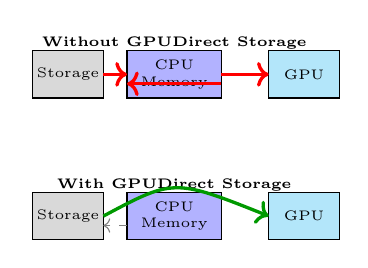
\begin{tikzpicture}[scale=0.6, every node/.style={font=\tiny}]
% Without GPUDirect Storage
\node[anchor=north] at (3,6) {\textbf{Without GPUDirect Storage}};
\draw[fill=gray!30] (0,4.5) rectangle (1.5,5.5);
\node at (0.75,5) {Storage};
\draw[fill=blue!30] (2,4.5) rectangle (4,5.5);
\node[align=center] at (3,5) {CPU\\Memory};
\draw[fill=cyan!30] (5,4.5) rectangle (6.5,5.5);
\node at (5.75,5) {GPU};

\draw[->, red, very thick] (1.5,5) -- (2,5);
\draw[->, red, very thick] (4,5) -- (5,5);
\draw[->, red, very thick] (4,4.8) -- (2,4.8);

% With GPUDirect Storage
\node[anchor=north] at (3,3) {\textbf{With GPUDirect Storage}};
\draw[fill=gray!30] (0,1.5) rectangle (1.5,2.5);
\node at (0.75,2) {Storage};
\draw[fill=blue!30] (2,1.5) rectangle (4,2.5);
\node[align=center] at (3,2) {CPU\\Memory};
\draw[fill=cyan!30] (5,1.5) rectangle (6.5,2.5);
\node at (5.75,2) {GPU};

\draw[->, green!60!black, very thick] (1.5,2) .. controls (3,2.8) .. (5,2);
\draw[->, gray, dashed] (2,1.8) -- (1.5,1.8);
\end{tikzpicture}
\end{column}
\end{columns}
\end{frame}

\begin{frame}{Multi-Instance GPU (MIG)}
\begin{columns}
\begin{column}{0.5\textwidth}
\textbf{Isolation and QoS mechanism}

\textbf{Each instance gets its own:}
\begin{itemize}
    \item Cores
    \item On-chip memory and cache
    \item Memory bandwidth
\end{itemize}

\textbf{GPU can be partitioned into different-sized MIG instances}

\textbf{Dynamically reconfigurable}

\vspace{0.3cm}
\textbf{Limitations:}
\begin{itemize}
    \item Limited \# of instances
    \item Resources are proportionally fixed
\end{itemize}
\end{column}

\begin{column}{0.45\textwidth}
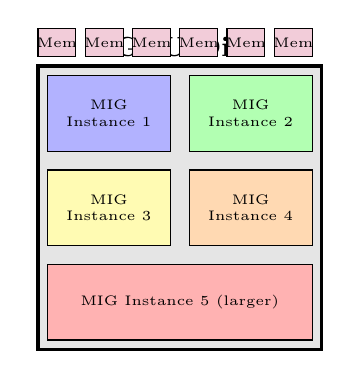
\begin{tikzpicture}[scale=0.6]
% GPU die
\draw[very thick, fill=gray!20] (0,0) rectangle (6,6);
\node[anchor=south] at (3,6) {\textbf{GPU Die}};

% MIG instances
\draw[fill=blue!30] (0.2,4.2) rectangle (2.8,5.8);
\node[align=center, font=\tiny] at (1.5,5) {MIG\\Instance 1};

\draw[fill=green!30] (3.2,4.2) rectangle (5.8,5.8);
\node[align=center, font=\tiny] at (4.5,5) {MIG\\Instance 2};

\draw[fill=yellow!30] (0.2,2.2) rectangle (2.8,3.8);
\node[align=center, font=\tiny] at (1.5,3) {MIG\\Instance 3};

\draw[fill=orange!30] (3.2,2.2) rectangle (5.8,3.8);
\node[align=center, font=\tiny] at (4.5,3) {MIG\\Instance 4};

\draw[fill=red!30] (0.2,0.2) rectangle (5.8,1.8);
\node[align=center, font=\tiny] at (3,1) {MIG Instance 5 (larger)};

% Memory sections
\foreach \i in {0,...,5} {
    \draw[fill=purple!20] (\i*1,6.2) rectangle (\i*1+0.8,6.8);
    \node[font=\fontsize{5}{6}\selectfont] at (\i*1+0.4,6.5) {Mem};
}
\end{tikzpicture}
\end{column}
\end{columns}
\end{frame}

\section{Conclusion}

\begin{frame}{Conclusion}
\begin{itemize}
    \item GPUs provide massive parallelization
    \item Has unique challenges in compute due to scheduling (divergence)
    \item Encounters similar challenges to CPU when it comes to memory, I/O
    \item Slowly turns into a ``first-class citizen''
\end{itemize}

\vspace{1cm}
\begin{center}
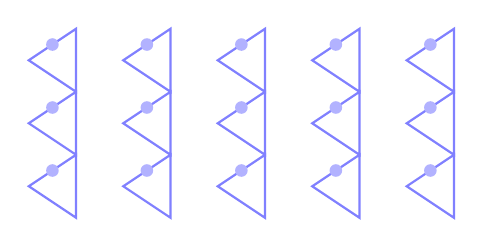
\begin{tikzpicture}
\foreach \i in {0,...,4} {
    \foreach \j in {0,...,2} {
        \draw[blue!50, thick] (\i*1.2,\j*0.8) -- ++(0.6,0.4) -- ++(0,-0.8) -- cycle;
        \fill[blue!30] (\i*1.2+0.3,\j*0.8+0.2) circle (0.08);
    }
}
\end{tikzpicture}
\end{center}
\end{frame}

\end{document}
